\documentclass{article}

% if you need to pass options to natbib, use, e.g.:
%     \PassOptionsToPackage{numbers, compress}{natbib}
% before loading neurips_2019


% to compile a camera-ready version, add the [final] option, e.g.:
\usepackage[nonatbib]{neurips_2019}

% to avoid loading the natbib package, add option nonatbib:
%     \usepackage[nonatbib]{neurips_2019}

\usepackage{natbib}

\usepackage[utf8]{inputenc} % allow utf-8 input
\usepackage[T1]{fontenc}    % use 8-bit T1 fonts
\usepackage{hyperref}       % hyperlinks
\usepackage{url}            % simple URL typesetting
\usepackage{booktabs}       % professional-quality tables
\usepackage{amsfonts}       % blackboard math symbols
\usepackage{nicefrac}       % compact symbols for 1/2, etc.
\usepackage{microtype}      % microtypography
\usepackage{xcolor}
\usepackage{graphicx}
\title{Continual learning in the game development context\\Collaboration with La Forge, Ubisoft }

\newcommand{\sarath}[1]{\textcolor{red}{[Sarath: #1]}}
\newcommand{\Mat}[1]{\textcolor{cyan}{[Mat: #1]}}
\newcommand{\mat}[1]{\textcolor{cyan}{[Mat: #1]}}
\newcommand{\Do}[1]{\textcolor{green}{[Do: #1]}}


\begin{document}

\maketitle

\textbf{Project Lead(s) (unordered):} Doriane Olewicki.

\textbf{Members (unordered):} Sarath Chandar, Mathieu Nayrolles, Olivier Pomarez, Mojtaba.

\textbf{Research Area (keywords):} Continual learning in software engineering, Continuous integration.

\section{Motivation}

%Explain the motivation for the project.

In the game industry, software projects extend over several years: for instance, a typical AAA game is developed for 3 to 5 years. To make the development process easier for the developers, tools are put at their disposal to help with, for instance, the artistic creation process or code integration. Those tools are based on machine learning (ML) models and learning processes, trained on historical data.

While such ML models might work accurately right after training, their predictions might lose relevance as time goes by, since the project's development objectives change over time, becoming progressively different from those at the time of model training. The phenomena of models and dataset aging are referred to as concept drift in the literature.

Through this research, we want to study concept drift in the game industry using the years of historical data and tool performance Ubisoft has gathered over time. Better understanding of concept drift would allow game tool creators to decide strategically when to update learning processes, and with which dataset, in order to maximize the performance of the tools over a long period of time. Furthermore, we want to apply techniques of continual learning to improve the performance and reduce the concept drift impact on those processes.

\section{Problem Statement}

%\begin{itemize}
%    \item Write a clear problem statement.
%    \item List the baselines that you should compare with.
%    \item Explain the dataset or environment you will be using.
%    \item Explain the metrics that you should use for the comparison.
%\end{itemize}  


We aim at automating the updates of machine learning models used in the context software products such as game development tools. To do so, we identified three research questions: 

\begin{description}
	\item[RQ1]: Can we accurately determine when to retrain/update a learning process, based on the performance of the model or changes in the data’s behavior over time? 
	\item[RQ2]: Can we accurately determine the dataset to use for re-training/updating a learning process to improve the process’ performance while reducing the training dataset size?
	\item[RQ3]: Can we maintain the learning process’ performance when the use-cases switch to another development phase or during and after punctual events/accidents?
\end{description}

The project is done in collaboration with La Forge, Ubisoft Montréal. They provide us with access to several product used in a large range of projects. To begin with, we start with a dataset used for the BrownBuild initiative, which is composed of build log files. This initiative aimed at identifying unreliable (brown) build jobs.  The BrownBuild project is runned on six different projects at the moment. Those projects differ in language, purposes and build activity.

Concept drift analysis was already started in that initiative (see: BrownBuild paper). The prototype proposed by the initiative uses a XGBoost model. We analysed in the initiative when to retrain the model and what window of data works best for it. This allowed us to keep the F1-score about 2-3 times higher than the baseline used in that project. 
The baseline that were used in the BrownBuild initiative are discribed in Table~\ref{brownbuild:baselines}



\begin{table*}[h!]
	\centering
	\caption{\label{brownbuild:baselines} Baselines for the BrownBuild initiative (with $BFR$ the brown failure ratio by project). }
	\begin{tabular}{|r|l|l|l|l|l|}
		\hline
		\\[-1em]
		\textbf{Baseline name}& \textbf{Chances of brown prediction}& \textbf{Precision} & \textbf{Recall} & \textbf{Specificity} & \textbf{F1-score}\\
		\hline
		\\[-1em]
		Random50   &50\%&$BFR$&$\frac{1}{2}$&$\frac{1}{2}$&$\frac{1}{\frac{1}{BFR}+2} = \frac{BFR}{1+2BFR}$\\%\\[-1em]
		RandomB    &$BFR$\%&$BFR$&$BFR$          &$1-BFR$&$\frac{1}{\frac{1}{BFR}+\frac{1}{BFR}} = \frac{BFR}{2}$\\%\\[-1em]
		AlwaysBrown&100\%&$BFR$&$1$          &$0$&$\frac{1}{\frac{1}{BFR}+1} = \frac{BFR}{1+BFR}$\\			
		\hline
	\end{tabular}
\end{table*}


For this new project, we aim at using concepts of continual learning to improve the BrownBuild initive's performances (F1-score). The first step is thus to switch the XGBoost model to a Neural Network model with similar or better performances. Since Neural Network are incremental learning processes, we are able to update the model without having to recompute it from scratch.

New baselines are identified at this point. 
\begin{itemize}
	\item 
\end{itemize}

%Our two objectives consider two equivalent, complementary approaches to deal with concept drift: (1) choosing the right time to retrain models, and (2) choosing models and learning algorithms that are more efficient at being retrained.
%From now on, when we will refer to the performance of a model, we will refer to the metric used to validate said model (i.e. accuracy, precision, recall). 
%
%
%\subsection{Obj. 1: Determining the optimal model \& data TTL (Time-to-live)}
%
%With learning processes, in the extreme case, each prediction could ask for a new model training to have the latest data included. However, this is not realistic, since training a model takes time and would increase the prediction time. If many predictions need to be made in a day, this could jam the project’s pipeline. Hence:
%
%\begin{itemize}
%	\item Usually, a model has to be used for several predictions, but this brings a new problem to the prediction: how long does my model stay relevant ? This corresponds to determining the model's TTL (time-to-live). The longer the TTL, the lower the frequency of model retraining, but the higher the risk of outdated predictions..
%	\item A related issue is that we also need to identify how long data stays relevant and when old data should be discarded. Data can get outdated by the project changing over time. Also some periods and events during the development might not be relevant to keep in the dataset, depending on the current situation. Finally, depending on the complexity of the learning algorithm, large training sets require more resources for the training process.
%\end{itemize}
%We want to identify when a model should be updated or retrained and which part of the data should be removed from the training set, taking into account the presence of cyclic behavior and punctual events.
%
%By identifying the time in the life of a project, as well as the aging of the data and the model, we would select more wisely what to use for the next training and when to do it.
%
%\subsection{Obj. 2: Applying continual learning techniques to learning processes}
%
%With neural networks, models can be incrementally updated with new data. The study of continual learning is an existing domain studying how the performance of a model evolves across time while new data is added to the training over time. Continual learning does not need a full retraining when the model needs to be updated, which reduces the computation time of model updating. Different continual learning techniques of model updates have been studied in the literature regarding what data to use and how to manage changes in the learning process.
%
%However, existing work on continual learning mostly refers to models where new tasks are added overtime, or new classes to identify. In contrast, our use-cases are still learning the same task and the same classes over time. however, since the use-cases show drifting in the dataset’s distribution, the task evolves over time. The use of continual learning promises to improve prediction performance in case of concept drift, while keeping model updates short (incremental), especially when the updates could be done strategically and with the right data observations, using the findings of Objective 1.

\section{Most Related Work}

%You should maintain a list of most related work to the project. This is not like the related work section in conference papers (even though we will use this section to write the related work section in the resulting conference paper). If you add a paper in this section, it means that you have read that paper in detail. To maintain a list of papers related to the project that you want to read in future, see \textit{literature.tex}.
%
%You should have a subsection for each related paper. I have given a sample subsection here. Follow the same format.
%
%\subsection{\citet{Chandar-2019}}
%
%Sarath Chandar*, Chinnadhurai Sankar*, Eugene Vorontsov, Samira Ebrahimi Kahou, Yoshua Bengio. \textit{Towards Non-saturating Recurrent Units for Modelling Long-term Dependencies.} Proceedings of AAAI, 2019.
%
%\begin{itemize}
%    \item Few line summary of the work.
%    \item Few line explanation of their results including datasets or environments used.
%    \item Explain how it is related to this project and this project is different from this work.
%\end{itemize} %similar work
\section{Model and Experiments}

%This section is a mix of models and experiments. This is the main section of the report which will log the entire research process. You will write down the precise description of the model, experiment design, results, graphs, analysis of results, next set of experiments, and so on.
%
%As the model evolves over time, do not edit the already described model. Write a new version of the model. Treat this section as a research log. Not as a research paper.
%
%Use the images folder to put all your images. Use \textit{meetings.tex} to maintain a log of all the project meetings and weekly to-do list.

\subsection{Neural network version of BrownBuild}

The BrownBuild initiative classifies failed builds as being brown (unreliable) or safe (true failures). This binary classification is based on a XGBoost classifier. 
To be able to apply Continual learning approaches, the first step is transform the classification model into a Neural Network (NN): in fact, NN can be used in online learning, so that updates can be done while the model is used instead of retraining from scratch when a modification in needed.

\Do{add parameters tested}

\Do{add final results for this part}

\subsection{Continual learning with a NN model for BrownBuild detection}

We know have to define a Continual Learning set-up for the project. 


\begin{figure}[h]
    \centering
    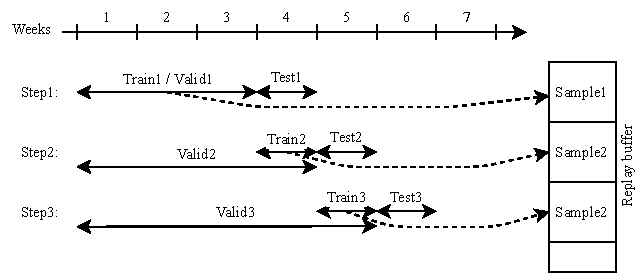
\includegraphics{img/CLUbi_sets.pdf}
    \caption{Set-up of the different sets during the Continual Learning process.}
    \label{fig:CL_set_setup }
\end{figure}
% This need to be compared to the results of concept drift that was computed in the BrownBuild paper (ADD REF). 


\section{Significant Results}

%This section is basically a summary of the previous section. Summarize the main findings of the project here. At any point of time in the course of the project, if you get a significant result which you think is one of the important findings of the project, copy it from previous section to this section (copy-paste, not cut-paste).
%
%The main advantage of this section is that, you can comment out the previous section at any point and then you have a nice summary of the project (which could be used to explain the project to others).
\section{Future Ideas}

%Use this section to write down all the future ideas based on this project. If you think about an extension which is out of scope for the current project, write it down here before you forget it.

\bibliography{refs}
% \bibliographystyle{acl_natbib}
\bibliographystyle{apalike}
\end{document}
